\section{Esperimenti}
In questa sezione vengono riportati gli esperimenti effettuati per l'aspect-based sentiment analysis sui due modelli ASUM e JST. Per i due modelli sono state utilizzate le implementazioni degli autori\footnote{\url{https://yohanjo.github.io/research/WSDM11/index.html}}\footnote{\url{https://github.com/linron84/JST}}.

I modelli sono stati valutati tramite il task di \textit{sentiment classification}, poiché non è disponibile nessuna \textit{groundtruth} per valutare i \textit{senti-aspects}.

Come \textit{groundtruth} per la \textit{sentiment classification} sono state considerate le valutazioni in ``stelle'' date dai recensori. I valori 1 e 2 sono stati considerati avere \textit{sentiment} negativi, mentre 4 e 5 positivi. I valori 3 sono stati esclusi dalla valutazione poiché il \textit{sentiment} neutrale non è stato modellato.

Per ogni esperimento sono state effettuate 10 prove e sono stati mediati i risultati in termini di F1-macro, poiché il \textit{sentiment} è sbilanciato.
% TODO: Motivare F1-macro 

Gli esperimenti che sono stati effettuati considerano diversi metodi di normalizzazione dei token (lemmatization, stemming, raw) e un diverso numero di topic (10, 20, 30, 50), mentre i parametri dei modelli (alpha, beta e gamma) sono stati fissati come nei lavori originali \cite{jo2011aspect}, \cite{lin2009joint}.

Per limitazioni di risorse computazionali ci si è limitati a effettuare gli esperimenti sulla normalizzazione solo per ASUM, poiché nell'implementazione usata viene fornita la possibilità di eseguire in \textit{multi-thread}, mentre per JST è stato considerato solo il caso con \textit{stemming}.


\subsection{ASUM}
%, diversi numeri di topic sono stati considerati 10, 20, 30 e 50, mentre il resto dei parametri sono stati %fissati come fatto nel lavoro originale alpha = 0.1, beta = [0.001, 0.1, 0] e gamma = [1, 1].

Come si può vedere nella figura \ref{fig:asum_normalization} il metodo di normalizzazione migliore risulta essere \textit{stemming} seguito da \textit{lemmatization}, mentre il caso senza normalizzazione risulta quello peggiore.
%
In generale all'aumentare del numero di topic si hanno valori di F1 più alti e una variabilità prove più bassa tra le 10.

\begin{figure}[ht]
  \centering
  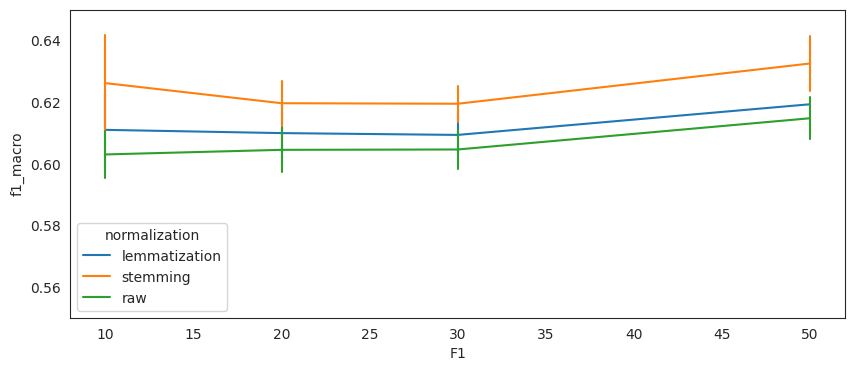
\includegraphics[width=0.95\textwidth]{images/experiments/asum_normalization.png}
  \caption{F1 al variare della normalizzazione e del numero di topic per ASUM.}
  \label{fig:asum_normalization}
\end{figure}

\newpage
\subsection{Comparazione ASUM e JST}
Successivamente sono state effettuate le prove con JST al variare del numero di topic con solo stemming.
%
Confrontando ASUM e JST figura (\ref{fig:asum_vs_jst}) è possibile notare come a prescindere dal numero di topic considerato ASUM ottenga risultati superiori in termini di F1 rispetto a JST.

La prova con valore di F1 più alto viene scelta come modello finale ovvero ASUM considerando 50 topic effettuando stemming con 63.8\% di F1.

\begin{figure}[ht]
  \centering
  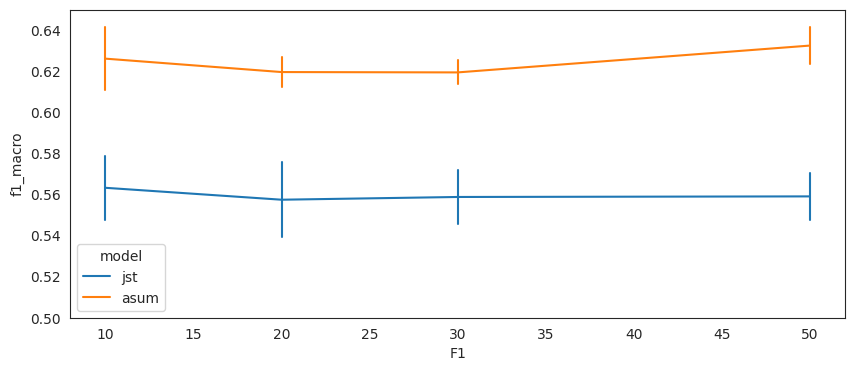
\includegraphics[width=0.95\textwidth]{images/experiments/asum_vs_jst.png}
  \caption{Comparazione di ASUM e JST sul task di sentiment classification al variare del numero di topic e usando stemming come normalizzazione.}
  \label{fig:asum_vs_jst}
\end{figure}

\subsection{Negazione dei token}
Infine un'ulteriore prova è stata effettuata per cercare di migliorare i risultati di ASUM.
Sotto assunzione che le congiunzioni avversative siano il punto in cui cambi l'opinione della frase, ogni frase è stata separata considerando le seguenti congiunzioni: "but, still, yet, while, however, nevertheless, whereas, notwithstanding, although e even though", in modo da migliorare la fase di negazione dei token.

\begin{figure}[ht]
    \centering
    
    \begin{quote}
    \begin{mdframed}
        \textbf{Text:} It's a very nice unit and great performance for the price point, however the fan noise was too loud for me.
        
        \textbf{Tokens (without split conjunctions):} ['nice', 'unit', 'great', 'performance', 'price', 'point', 'fan', 'noise', 'loud']

        \textbf{Tokens (with split conjunctions):} [['nice', 'unit', 'great', 'performance', 'price', 'point'], ['not\_fan', 'not\_noise', 'not\_loud']]

    \end{mdframed} 
    \end{quote}
    
    \caption{Effetto della separazione di frasi utilizzando le congiunzioni sulla negazione dei token. A scopi visualizzativi in questo esempio viene utilizzata la lemmatization.}
    \label{fig:tokens-negation-example}
\end{figure}

\begin{figure}[ht]
  \centering
  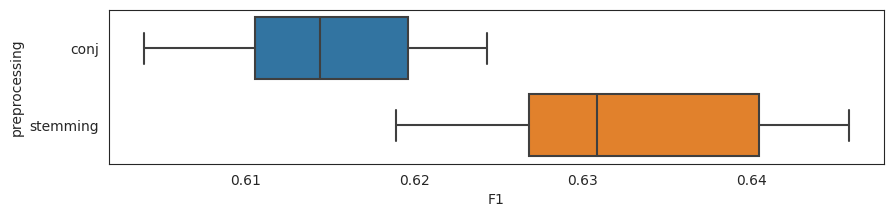
\includegraphics[width=0.95\textwidth]{images/experiments/conj_exp.png}
  \caption{Comparazione del modello migliore con il metodo che sfrutta le congiunzioni avversative.}
  \label{fig:asum_conj}
\end{figure}

\newpage
Considerando la figura \ref{fig:asum_conj} è possibile vedere che la modifica proposta addirittura comporta un peggioramento nella classificazione del sentiment, contrariamente da quanto aspettato, perciò tale modifica non verrà considerata per l'estrazione dei topic.

\subsection{Identificazione Topics}
Per ognuno dei 100 \textit{senti-aspect} sono state assegnate delle etichette considerando le top-10 parole più probabili in ogni \textit{senti-aspect}, successivamente verranno riportati alcuni esempi di topic con le relative etichette assegnate.

Alcuni \textit{senti-aspect} che sono stati individuati corrispondono allo
stesso concetto e hanno molte parole in comune, quindi sono state associate alla stessa etichetta, come ad esempio si può notare nelle figure \ref{fig:T3-CoolingSystem} e \ref{fig:T4-CoolingSystem}.

Quindi questi \textit{senti-aspect} sono stati aggregati in una partizione composta da 22 aspetti (figura \ref{fig:ttopics}).

\begin{figure}[ht]
  \centering
  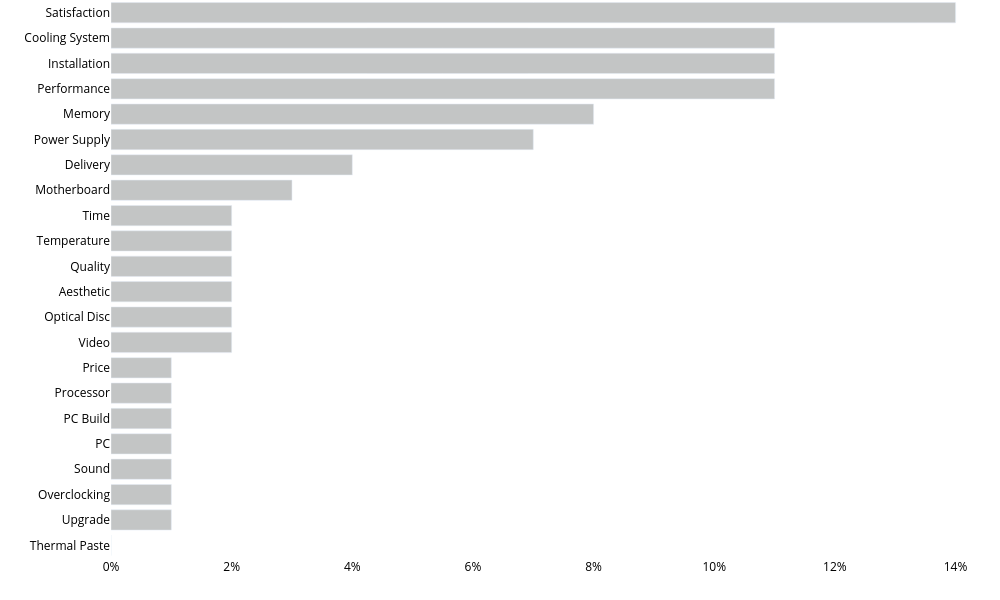
\includegraphics[width=\textwidth]{images/experiments/topics.png}
  \caption{Distribuzione delle recensioni per gli aspetti identificati.}
  \label{fig:ttopics}
\end{figure}

\begin{figure}[p]
  \centering
  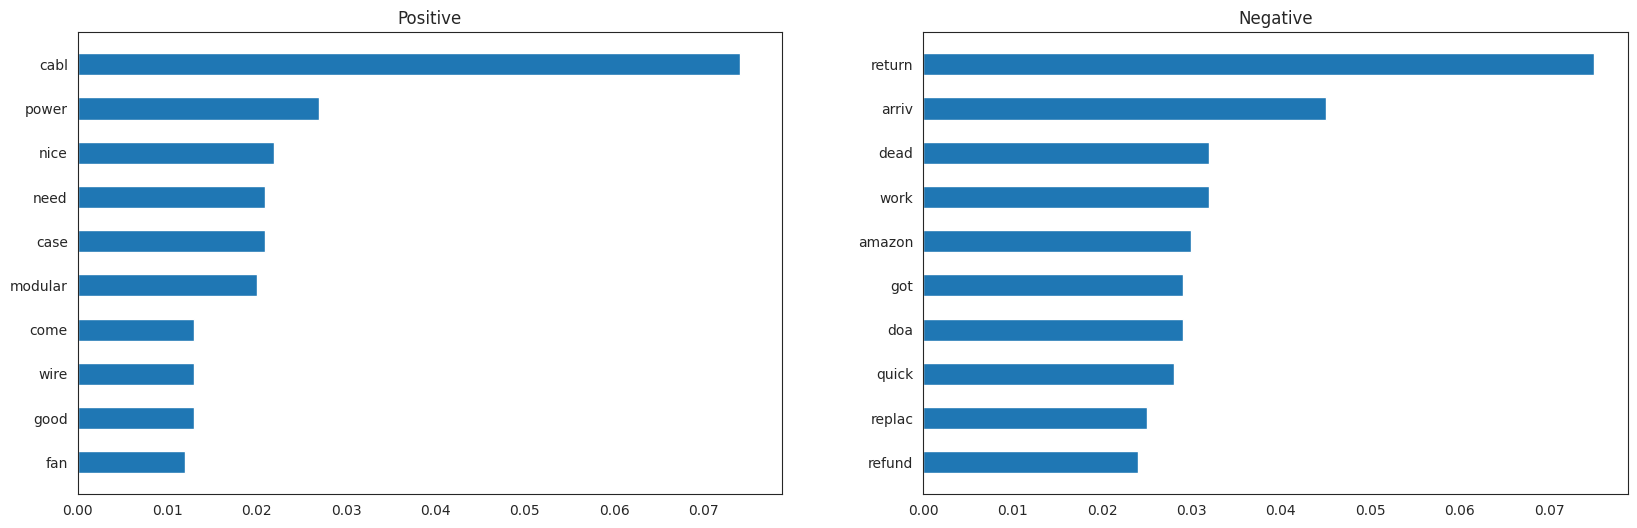
\includegraphics[width=0.95\textwidth]{images/experiments/T0-PSU.png}
  \caption{Power Supply}
  \label{fig:T0-PowerSupply}
\end{figure}

\begin{figure}[p]
  \centering
  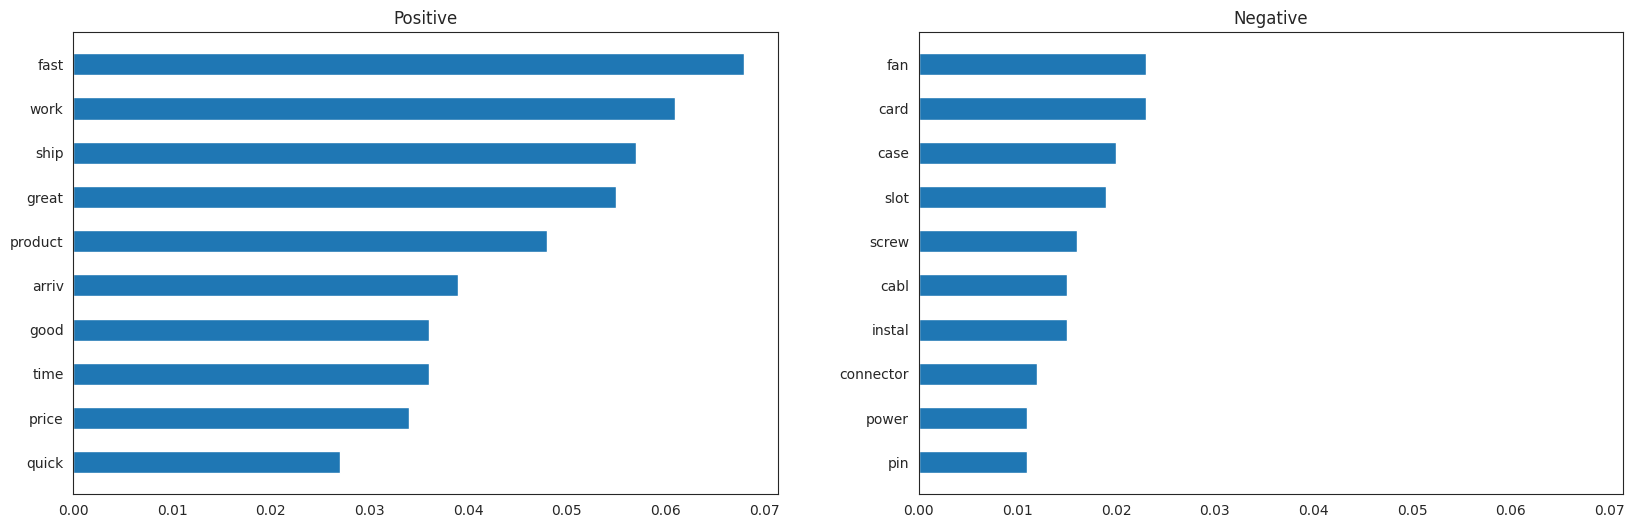
\includegraphics[width=0.95\textwidth]{images/experiments/T2-Delivery.png}
  \caption{Delivery}
  \label{fig:T2-Delivery}
\end{figure}

\begin{figure}[p]
  \centering
  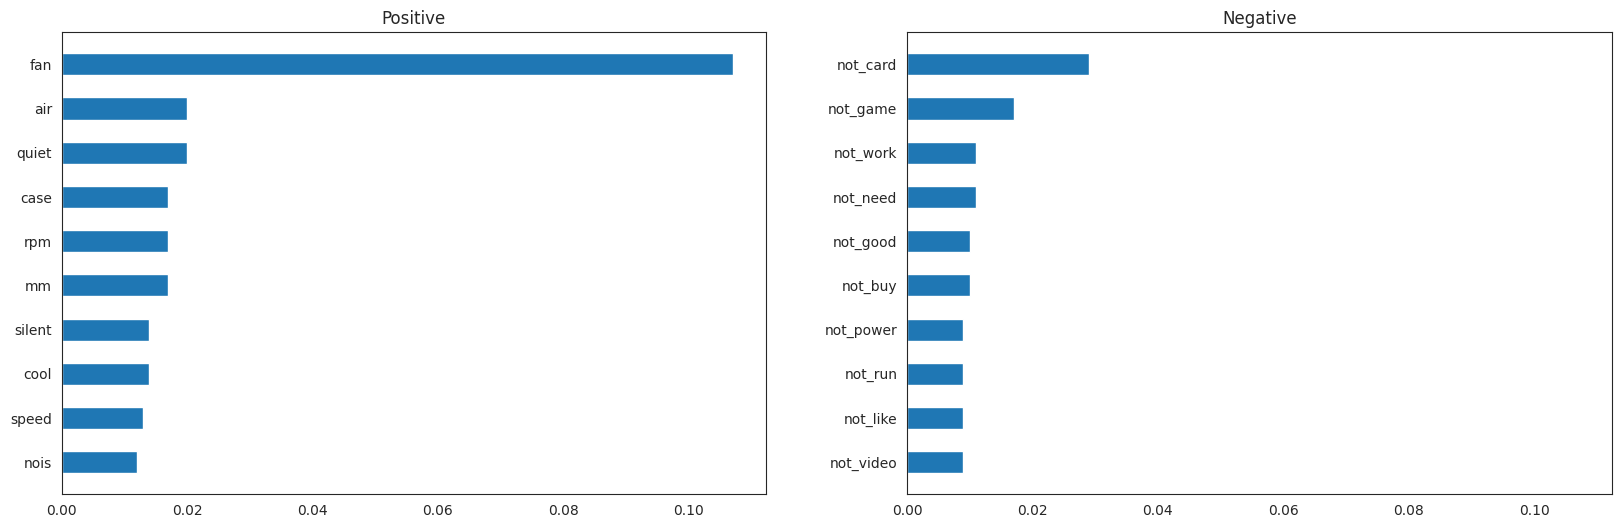
\includegraphics[width=0.95\textwidth]{images/experiments/T3-CoolingSystem.png}
  \caption{Cooling System}
  \label{fig:T3-CoolingSystem}
\end{figure}

\begin{figure}[p]
  \centering
  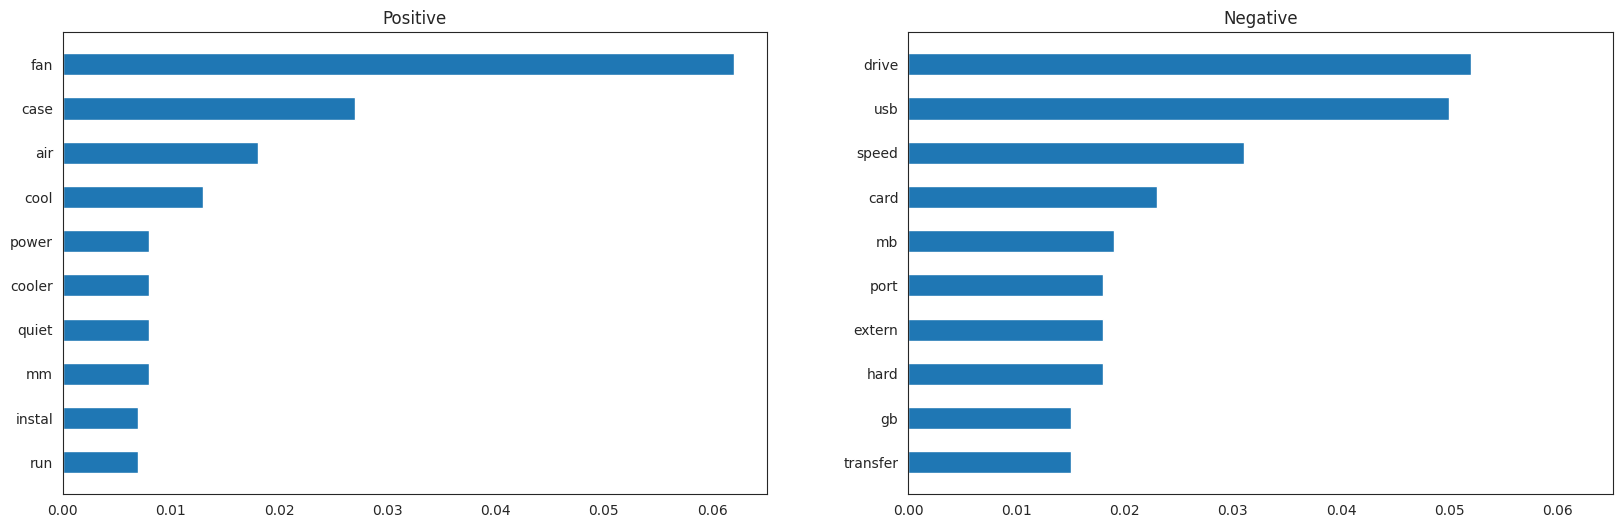
\includegraphics[width=0.95\textwidth]{images/experiments/T4-CoolingSystem.png}
  \caption{Cooling System}
  \label{fig:T4-CoolingSystem}
\end{figure}

\begin{figure}[p]
  \centering
  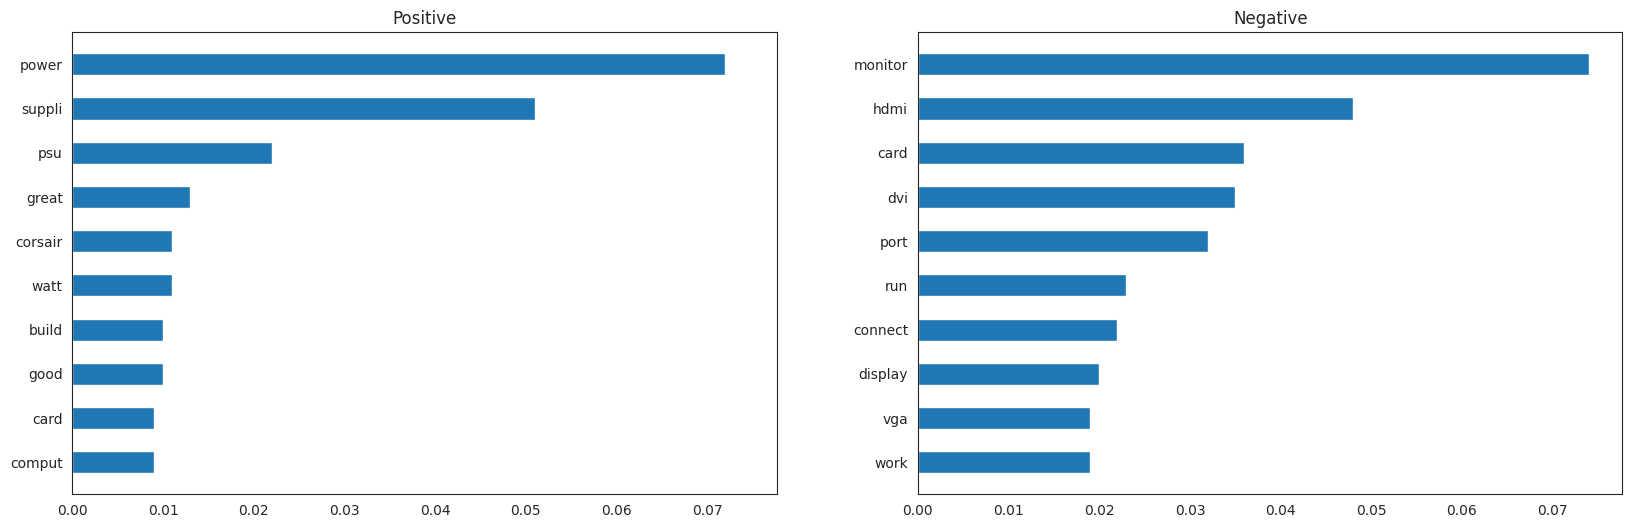
\includegraphics[width=0.95\textwidth]{images/experiments/T8-PSU.png}
  \caption{Power Supply}
  \label{fig:T8-PowerSupply}
\end{figure}

\begin{figure}[p]
  \centering
  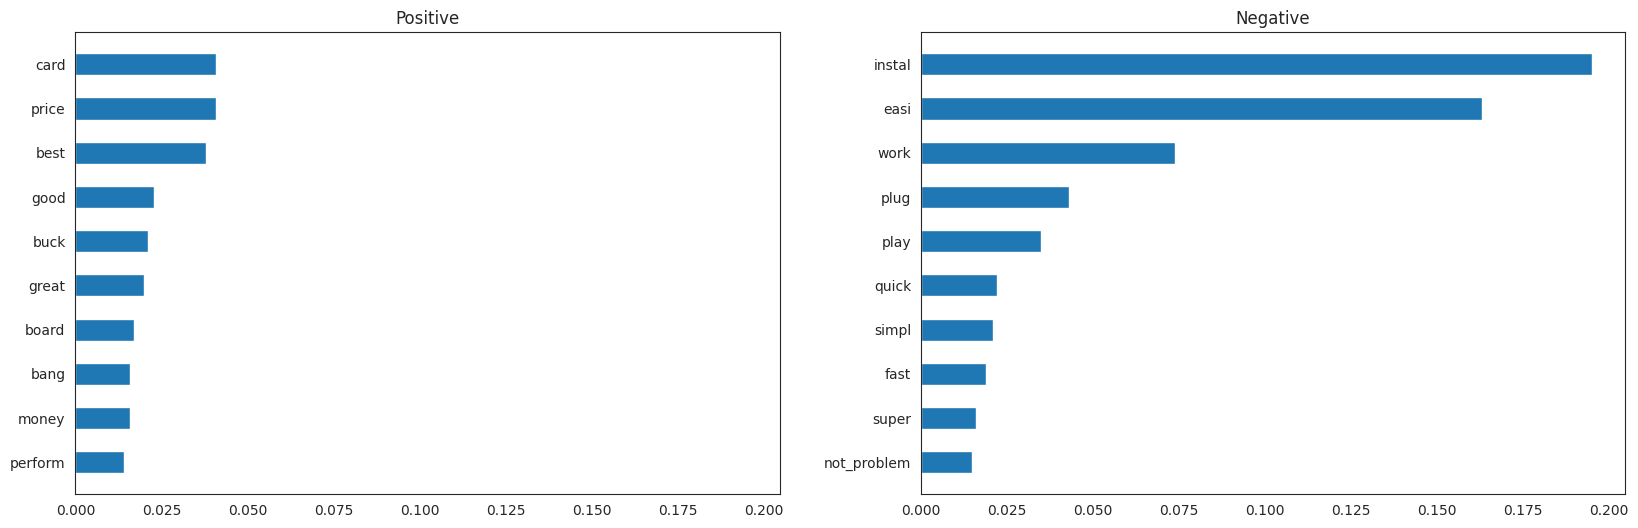
\includegraphics[width=0.95\textwidth]{images/experiments/T9-Price.png}
  \caption{Price}
  \label{fig:T9-Price}
\end{figure}

\begin{figure}[p]
  \centering
  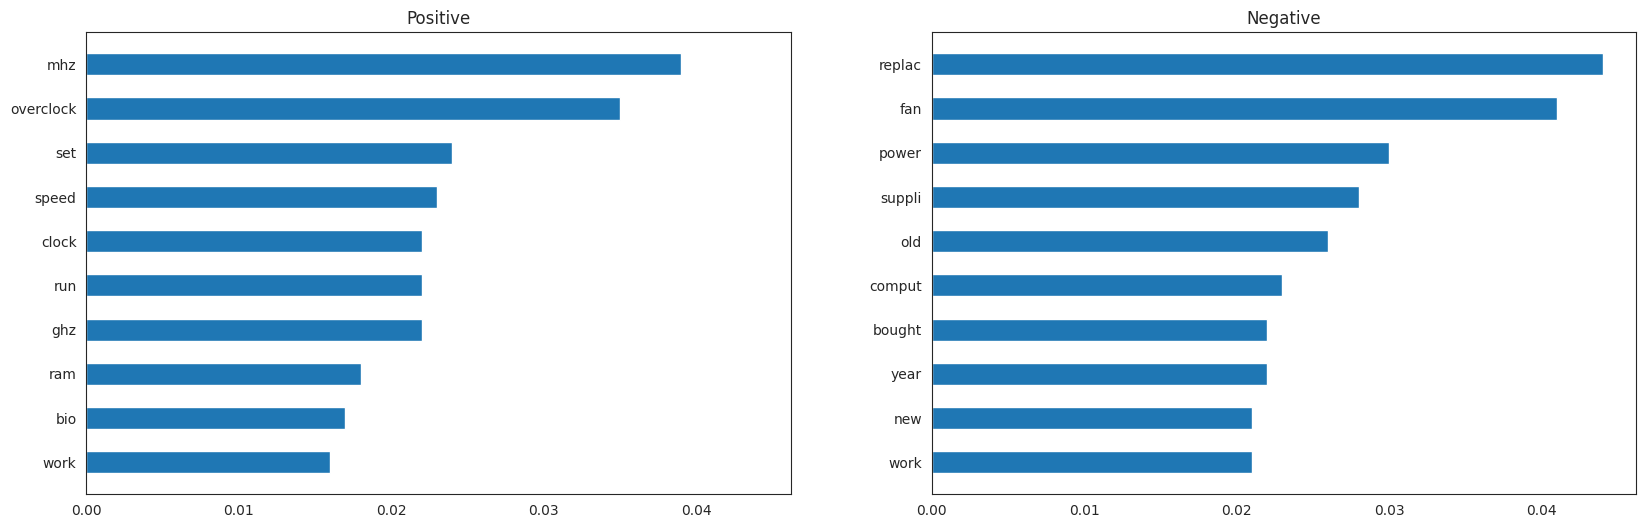
\includegraphics[width=0.95\textwidth]{images/experiments/T17-Overclocking.png}
  \caption{Overclocking}
  \label{fig:T17-Overclocking}
\end{figure}

\begin{figure}[p]
  \centering
  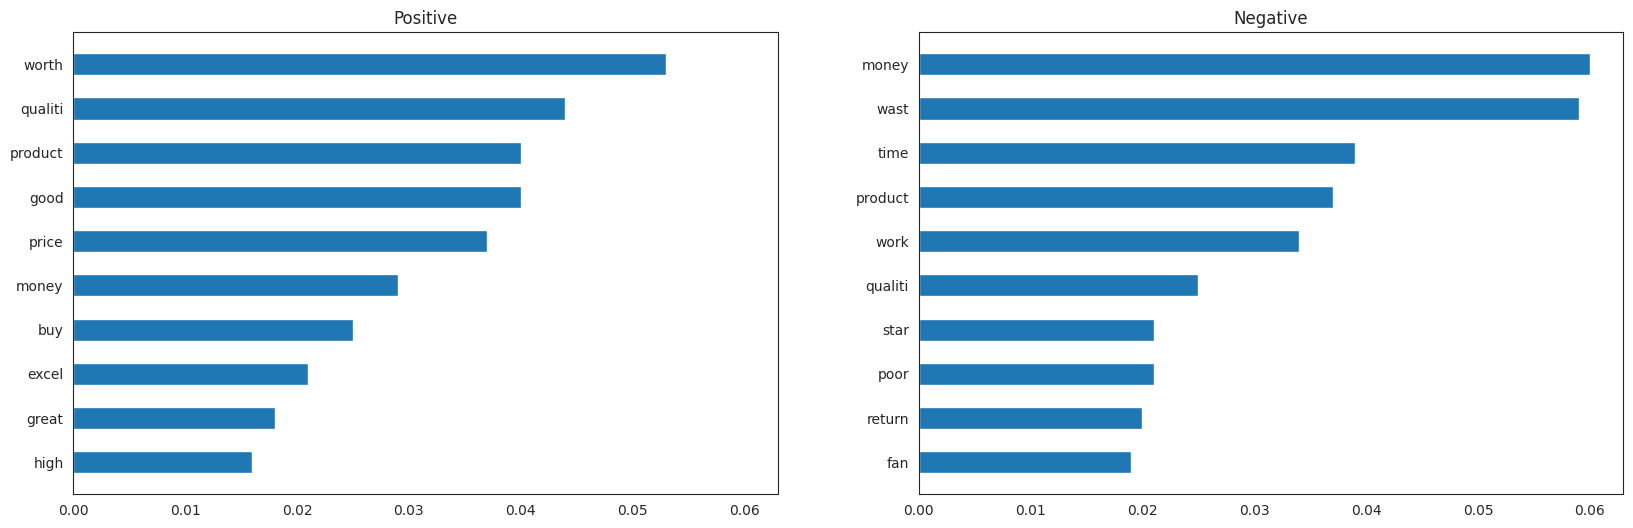
\includegraphics[width=0.95\textwidth]{images/experiments/T26-Quality.png}
  \caption{Quality}
  \label{fig:T26-Quality}
\end{figure}

\newpage

\begin{figure}[ht]
  \centering
  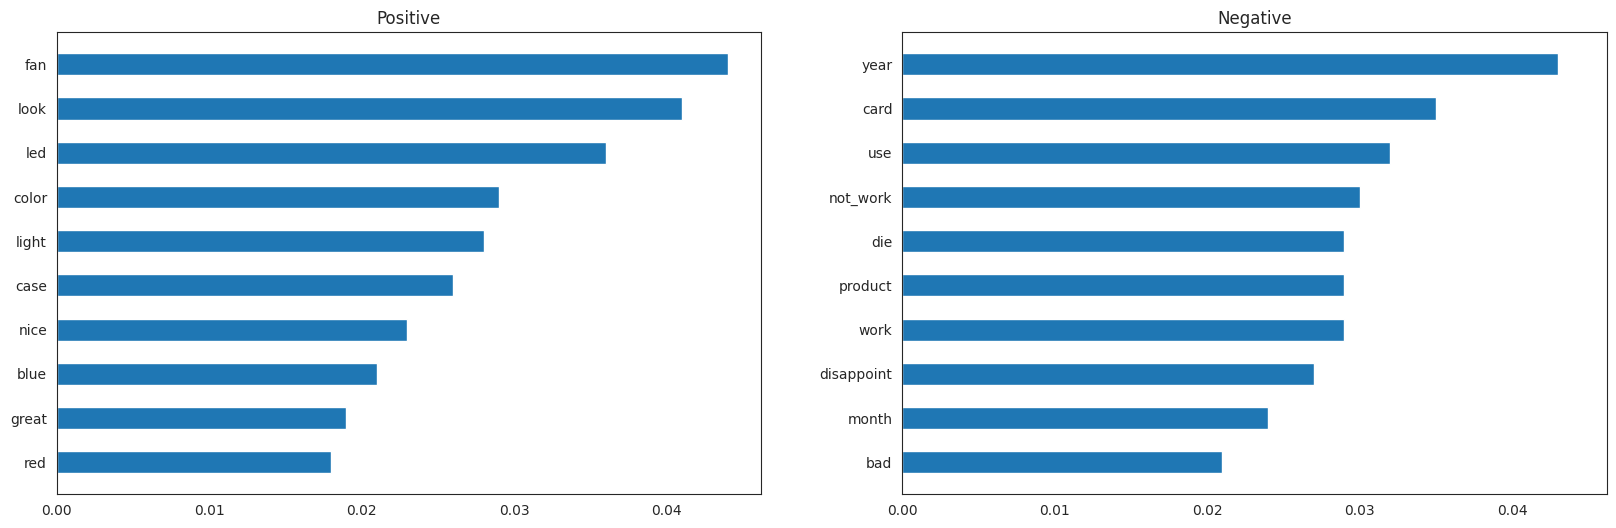
\includegraphics[width=0.95\textwidth]{images/experiments/T28-Aesthetic.png}
  \caption{Aesthetic}
  \label{fig:T28-Aesthetic}
\end{figure}

\begin{figure}[ht]
  \centering
  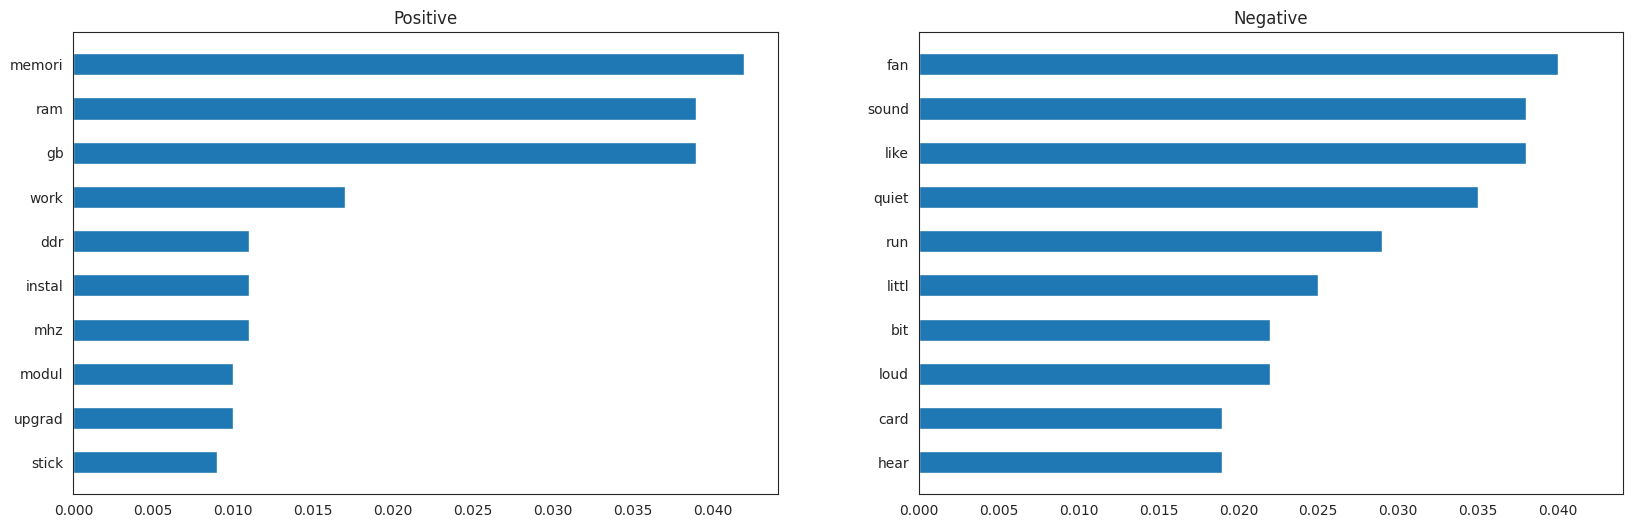
\includegraphics[width=0.95\textwidth]{images/experiments/T44-Memory.png}
  \caption{Memory}
  \label{fig:T44-Memory}
\end{figure}

\newpage

Per ogni recensione sono stati identificati i topic tramite una soglia $T$ sulla distribuzione di probabilità document-aspect.

I \textit{senti-aspect} che hanno una probabilità inferiore alla soglia $T$ non verranno considerati.
Inoltre le recensioni che presentano un'uguale probabilità per ogni topic fissato il sentiment non avranno assegnato alcun topic.

La scelta della soglia è stata effettuata manualmente in modo che abbia il valore più alto possibile tenendo topic con alta probabilità e che le recensioni abbiano un numero di topic maggiore possibile. Nella figura \ref{fig:T_soglia} viene comparato l'effetto di diverse soglie. 

\begin{figure}[ht]
  \centering
  \includegraphics[width=0.9\textwidth]{images/experiments/threshold_selection.png}
  \caption{In questo grafico sono riportati il numero medio di topic assegnati a una recensione in base al numero di frasi al variare di diversi valori di soglia.}
  \label{fig:T_soglia}
\end{figure}

La soglia è stata scelta considerando che ASUM assume che a ogni frase venga associato un aspetto.

La soglia è stata scelta superiore a 0.04545, ovvero il caso in cui tutti i \textit{senti-aspect} di una recensione hanno uguale probabilità, ed con il valore più alto possibile cercando di non scartarne troppi.

E' stata scelta una soglia di 0.075 che permette di avere un numero medio di circa 7 topic, considerando che il massimo numero di \textit{senti-aspect} assegnabile a una recensione è 44 avendo individuato 22 topic tra positivi e negativi, ma che è molto improbabile che appaiano tutti i 22 topic anche in recensioni con 50 frasi.
